\nsecbegin{Ziel des Sprints}

Das Ziel des Sprints ist das Abschließen mit dem Projekt. Es sollen die letzten Bugs gefixt werden, sodass die Version komplett lauffähig ist. Zum Projekt sollen noch Unittests hinzugefügt werden. Zudem soll die Präsentation vorbereitet und das Plakat erstellt werden.

\nsecend

\nsecbegin{User-Stories des Sprint-Backlogs}

\nsecbegin{Klassendiagramme}
Als Benutzer wünsche ich mir, Klassendiagramme aus meinem bestehenden Quellcode erstellen zu können, damit ich das nicht manuell tun muss.
\nsecend

\nsecbegin{Sequenzdiagramme}
Als Benutzer wünsche ich mir, Sequenzdiagramme aus meinem bestehenden Quellcode erstellen zu können, damit ich das nicht manuell tun muss.
\nsecend

\nsecbegin{Vorschau}
Als Benutzer wünsche ich mir eine Vorschau der Diagramme, damit ich einschätzen kann ob ich
damit zufrieden bin.
\nsecend

\nsecbegin{Anzeigen und Speichern von PlantUML}
Als Benutzer wünsche ich mir, Diagramme als PlantUML-Code anzeigen und speichern zu können, um den Aufbau nachvollziehen zu können.
\nsecend

\nsecend % {User-Stories des Sprint-Backlogs}

\nsecbegin{Zeitliche Planung}

Im ursprünglichen Plan sollte der Sprint vom 17.06. bis 27.06. gehen. Wobei später entschlossen wurde ihn auf den 05.07. zu erweitern. \\\\

\begin{figure}[hbtp]
	\centering
	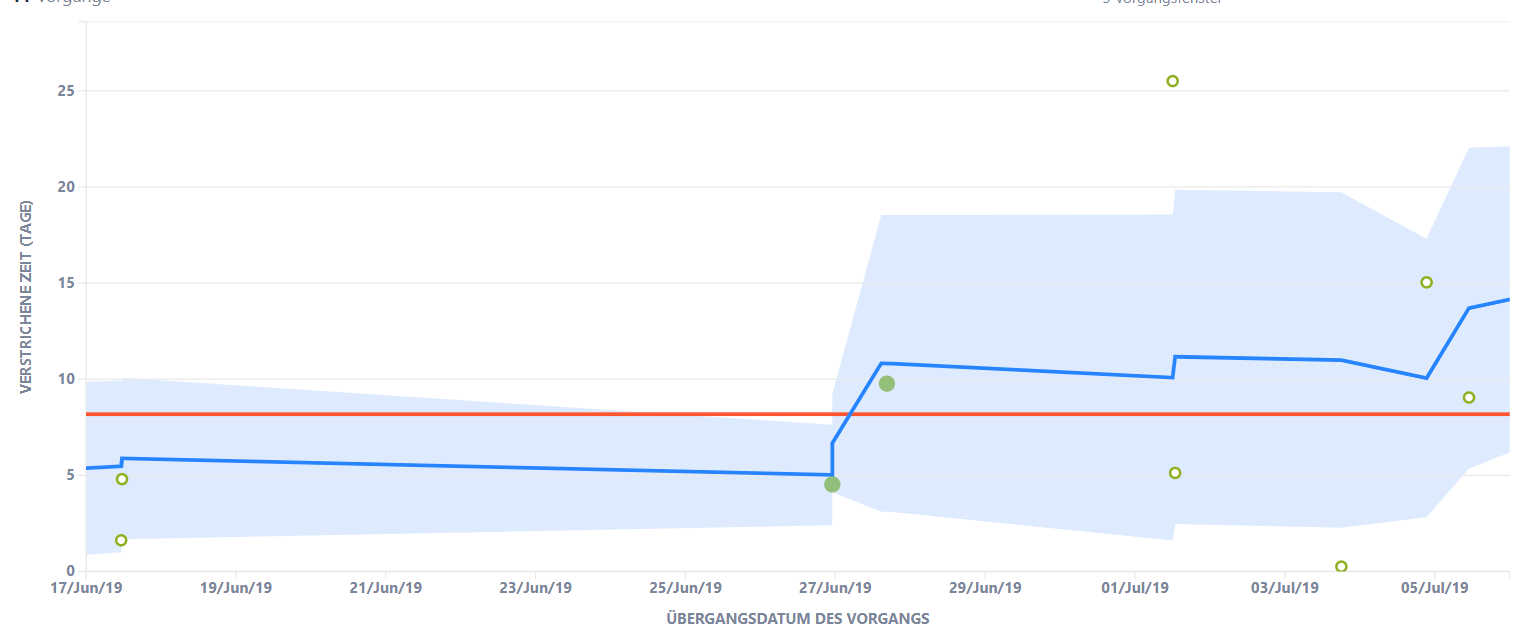
\includegraphics[width=\textwidth]{Bilder/ZeitSprint8}
	\caption{Zeit-Diagramm für Sprint 8}
\end{figure}

\nsecend%Zeitliche Planung

\nsecbegin{Liste der durchgeführten Meetings}

17.06. - Planung \\
21.06. - Meeting und dritte Zwischenstandspräsentation \\
24.06. - Meeting zum Zwischenstand und Plakatdesign \\
28.06. - Meeting (Sprint Verlängerung) \\
01.07. - Präsentationsplanung
05.06. - Vorstellung des Projekts und Review \\

\nsecend%Liste der durchgeführten Meetings

\nsecbegin{Ergebnisse des Planning-Meetings}

Es sollen die letzten Bugs gefixt werden und die Präsentation für die Vorstellung vorbereitet werden.
\\
Aufgaben für den Sprint:
\begin{itemize}
	\item GUI auflistung der Klassen und Methoden
	\item C++-Parser erstellen
	\item Unittest für Gesamtablauf mit Spezifikation
	\item Bugs in Parser fixen
	\item Code aufräumen
	\item Parser erweitern und Bugs fixen
	\item Umbau Logger
	\item Scaling fuer Graph img
	
\end{itemize}

\nsecend

\nsecbegin{Aufgewendete Arbeitszeit pro Person$+$Arbeitspaket}

\begin{longtable}{|p{4cm}|l|l|l|l|l|}
	\hline
	Arbeitspaket & Person & Start & Ende & h & Artefakt\\
	\hline	
	
	GUI  & Julian U.  & 17.06.2019 & 05.07.2019 & 6 & GUISwing.java \\ \hline
	C++ Parser erstellen & Jan S. & 17.06.2019 & 05.07.2019 & 26,5 & ParserCPP.java \\ \hline
	C++ Parser erstellen & Johann G.   & 17.06.2019 & 05.07.2019 & 26 & ClassDiagrammGenerator.java \\  & & & & & ParserCPP.java \\ \hline
	Unittest & Tore A.   & 17.06.2019 & 05.07.2019 &7 & OutputPUML.java \\ & & & & & GesamtTest.java  \\ \hline
    Java Parser  & Michael L.   & 17.06.2019 & 05.07.2019 & 21 & ParserJava.java \\ \hline
	Code aufräumen & Leo R.   & 17.06.2019 & 05.07.2019 & 2 & XmlHelperMethods.java \\ \hline
	Tests schreiben und Seq. Diag. & Leo R.   & 17.06.2019 & 05.07.2019 & 8 & SequenceDiagramGenerator.java \\ & & & & & SequenceDiagramGeneratorTest.java \\ \hline
	Java Parser & Jona M.   & 17.06.2019 & 05.07.2019 & 18 & ParserJava.java \\ \hline
	Umbau Logger & Patrick O.   & 17.06.2019 & 05.07.2019 & 6  & LogMain.java \\  & & & & & ParserJava.java \\& & & & & ParserCPP.java \\  \hline
	Scaling für Grafik & Patrick O.   & 17.06.2019 & 05.07.2019 & 0,5 & OutputPUML.java \\  \hline
	Plakat & Patrick O.   & 17.06.2019 & 05.07.2019 & 6 & - \\  \hline
	Console - Scaling & Marian G.  & 17.06.2019 & 05.07.2019 & 1,5 & Console.java\\ \hline
	Präsentation & Marian G.  & 17.06.2019 & 05.07.2019 & 2,5 & - \\ \hline
	Klassenauswahl & Marian G.  & 17.06.2019 & 05.07.2019 & 4 & Console.java \\ \hline
	Tests schreiben  & Elisabeth S.  & 17.06.2019 & 05.07.2019  & 5 & SequenceDiagramGeneratorTest.java \\ \hline
	Seq.Diag. anpassen  & Elisabeth S.  & 17.06.2019 & 05.07.2019  & 1,5 & SequenceDiagramGeneratorTest.java \\ \hline

\end{longtable}     

\nsecend

\nsecbegin{Konkrete Code-Qualität im Sprint}
Hat sich zum vorhergehenden Sprint kaum verändert.
\nsecend%Konkrete Code-Qualität im Sprint

\nsecbegin{Konkrete Test-Überdeckung im Sprint}
Die Testüberdeckung beträgt 52,1\% für den Quellcode des Projekts.
\nsecend%Konkrete Test-Überdeckung im Sprint

\nsecbegin{Ergebnisse des Reviews}

Es fand kein richtiges Review statt. Wir haben bei der Präsentation festgestellt, dass wir mit dem Ergebnis soweit zufrieden sind, auch wenn der Umstieg zwischen Java und CPP Parser noch nicht ohne Quellcodeänderungen funktioniert hat. Wir konnten unser ganzes Projekt parsen, die Begrenzung von PlantUML erschweren jedoch das darstellen von solch großen Projekten. Deshalb muss der erzeugte Quellcode in ein Online-PlantUML ohne diese Begrenzung eingegeben werden. Das ganze Projekt wurde soweit richtig geparsed.

\nsecend%Ergebnisse des Reviews

\nsecbegin{Abschließende Einschätzung des Product-Owners}
Insgesamt konnte das Produkt zu einem zufriedenstellenden Ausmaß finalisiert werden. Außer einzelner Bedienungseigenarten der GUI funktioniert das Erstellen von Klassen- und Sequenzdiagrammen für die definierten Testfälle intuitiv.
\nsecend%Abschließende Einschätzung des Product-Owners

\nsecbegin{Abschließende Einschätzung des Software-Architekten}
\begin{itemize}
\item Die nach Sprint 6 gesetzten Ziele wurden erreicht.
\item Der Logger ist weitestgehend integriert.
\item Die Kommandozeilenschnittstelle ist umfangreich.
\item Die GUI und das Betrachten der Diagramme darin funktioniert
\item Es sind aber noch einige kleinere Bugs und Unschönheiten vorhanden
\end{itemize}
\nsecend%Abschließende Einschätzung des Software-Architekten